% Important: If latex complains about unicode characters,
% please use "\usepackage[utf8x]{inputenc}" in your preamble
% You can change the size of the picture by putting it into the construct:
% 1) \resizebox{10cm}{!}{"below picture"} to scale horizontally to 10 cm
% 2) \resizebox{!}{15cm}{"below picture"} to scale vertically to 15 cm
% 3) \resizebox{10cm}{15cm}{"below picture"} a combination of above two
% It is not recomended to use the scale option of the tikzpicture environment.
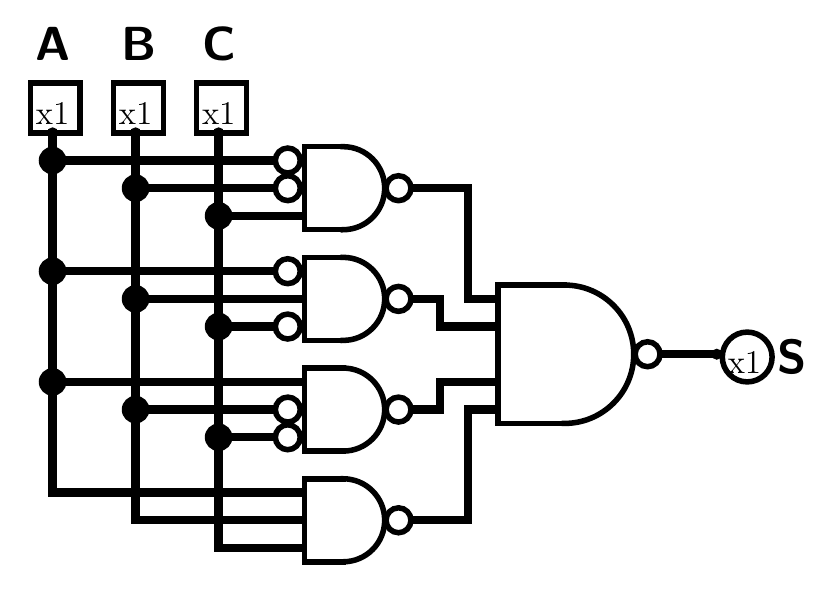
\begin{tikzpicture}[x=1pt,y=-1pt,line cap=rect]
\def\logisimfontA#1{\fontfamily{cmr}{#1}} % Replaced by logisim, original font was "SansSerif"
\def\logisimfontB#1{\fontfamily{Microsoft Sans Serif}{#1}}
\definecolor{custcol_0_0_0}{RGB}{0, 0, 0}
\definecolor{custcol_ff_ff_ff}{RGB}{255, 255, 255}
\draw [line width=3.0pt, custcol_0_0_0 ]  (45.0,46.0) -- (45.0,66.0) -- (95.0,66.0) ;
\draw [line width=3.0pt, custcol_0_0_0 ]  (75.0,46.0) -- (75.0,76.0) -- (105.0,76.0) ;
\draw [line width=3.0pt, custcol_0_0_0 ]  (45.0,66.0) -- (45.0,106.0) -- (105.0,106.0) ;
\draw [line width=3.0pt, custcol_0_0_0 ]  (105.0,136.0) -- (15.0,136.0) -- (15.0,176.0) -- (105.0,176.0) ;
\draw [line width=3.0pt, custcol_0_0_0 ]  (15.0,46.0) -- (15.0,56.0) -- (15.0,96.0) -- (15.0,136.0) ;
\draw [line width=3.0pt, custcol_0_0_0 ]  (95.0,146.0) -- (45.0,146.0) -- (45.0,186.0) -- (105.0,186.0) ;
\draw [line width=3.0pt, custcol_0_0_0 ]  (45.0,106.0) -- (45.0,146.0) ;
\draw [line width=3.0pt, custcol_0_0_0 ]  (75.0,76.0) -- (75.0,116.0) -- (75.0,156.0) -- (75.0,196.0) -- (105.0,196.0) ;
\draw [line width=3.0pt, custcol_0_0_0 ]  (75.0,116.0) -- (95.0,116.0) ;
\draw [line width=3.0pt, custcol_0_0_0 ]  (75.0,156.0) -- (95.0,156.0) ;
\draw [line width=3.0pt, custcol_0_0_0 ]  (235.0,126.0) -- (255.0,126.0) ;
\draw [line width=3.0pt, custcol_0_0_0 ]  (15.0,56.0) -- (95.0,56.0) ;
\draw [line width=3.0pt, custcol_0_0_0 ]  (15.0,96.0) -- (95.0,96.0) ;
\draw [line width=3.0pt, custcol_0_0_0 ]  (145.0,66.0) -- (165.0,66.0) -- (165.0,106.0) -- (175.0,106.0) ;
\draw [line width=3.0pt, custcol_0_0_0 ]  (145.0,186.0) -- (165.0,186.0) -- (165.0,146.0) -- (175.0,146.0) ;
\draw [line width=3.0pt, custcol_0_0_0 ]  (145.0,106.0) -- (155.0,106.0) -- (155.0,116.0) -- (175.0,116.0) ;
\draw [line width=3.0pt, custcol_0_0_0 ]  (145.0,146.0) -- (155.0,146.0) -- (155.0,136.0) -- (175.0,136.0) ;
\fill [line width=3.0pt, custcol_0_0_0]  (15.0,96.0) ellipse (5.0 and 5.0 );
\fill [line width=3.0pt, custcol_0_0_0]  (75.0,156.0) ellipse (5.0 and 5.0 );
\fill [line width=3.0pt, custcol_0_0_0]  (45.0,66.0) ellipse (5.0 and 5.0 );
\fill [line width=3.0pt, custcol_0_0_0]  (15.0,136.0) ellipse (5.0 and 5.0 );
\fill [line width=3.0pt, custcol_0_0_0]  (45.0,106.0) ellipse (5.0 and 5.0 );
\fill [line width=3.0pt, custcol_0_0_0]  (75.0,76.0) ellipse (5.0 and 5.0 );
\fill [line width=3.0pt, custcol_0_0_0]  (45.0,146.0) ellipse (5.0 and 5.0 );
\fill [line width=3.0pt, custcol_0_0_0]  (15.0,56.0) ellipse (5.0 and 5.0 );
\fill [line width=3.0pt, custcol_0_0_0]  (75.0,116.0) ellipse (5.0 and 5.0 );
\draw [line width=2.0pt, custcol_0_0_0] (200.0,151.0) arc (90.0:-90.0:25.0 and 25.0 );
\draw [line width=2.0pt, custcol_0_0_0 ]  (200.0,101.0) -- (176.0,101.0) -- (176.0,151.0) -- (200.0,151.0) ;
\draw [line width=2.0pt, custcol_0_0_0]  (230.0,126.0) ellipse (4.5 and 4.5 );
\draw [line width=2.0pt, custcol_0_0_0]  (266.0,127.0) ellipse (9.0 and 9.0 );
\logisimfontA{\fontsize{12pt}{12pt}\selectfont\node[inner sep=0, outer sep=0, custcol_0_0_0, anchor=base west] at  (259.0,133.0)  {x1};}
\logisimfontB{\fontsize{16pt}{16pt}\sffamily\fontseries{bx}\selectfont\node[inner sep=0, outer sep=0, custcol_0_0_0, anchor=base west] at  (277.0,133.0)  {S};}
\fill [line width=2.0pt, custcol_0_0_0]  (255.0,126.0) ellipse (2.0 and 2.0 );
\draw [line width=2.0pt, custcol_0_0_0]  (100.0,96.0) ellipse (4.5 and 4.5 );
\draw [line width=2.0pt, custcol_0_0_0]  (100.0,116.0) ellipse (4.5 and 4.5 );
\draw [line width=2.0pt, custcol_0_0_0] (120.0,121.0) arc (90.0:-90.0:15.0 and 15.0 );
\draw [line width=2.0pt, custcol_0_0_0 ]  (120.0,91.0) -- (106.0,91.0) -- (106.0,121.0) -- (120.0,121.0) ;
\draw [line width=2.0pt, custcol_0_0_0]  (140.0,106.0) ellipse (4.5 and 4.5 );
\draw [line width=2.0pt, custcol_0_0_0]  (100.0,146.0) ellipse (4.5 and 4.5 );
\draw [line width=2.0pt, custcol_0_0_0]  (100.0,156.0) ellipse (4.5 and 4.5 );
\draw [line width=2.0pt, custcol_0_0_0] (120.0,161.0) arc (90.0:-90.0:15.0 and 15.0 );
\draw [line width=2.0pt, custcol_0_0_0 ]  (120.0,131.0) -- (106.0,131.0) -- (106.0,161.0) -- (120.0,161.0) ;
\draw [line width=2.0pt, custcol_0_0_0]  (140.0,146.0) ellipse (4.5 and 4.5 );
\draw [line width=2.0pt, custcol_0_0_0]  (100.0,56.0) ellipse (4.5 and 4.5 );
\draw [line width=2.0pt, custcol_0_0_0]  (100.0,66.0) ellipse (4.5 and 4.5 );
\draw [line width=2.0pt, custcol_0_0_0] (120.0,81.0) arc (90.0:-90.0:15.0 and 15.0 );
\draw [line width=2.0pt, custcol_0_0_0 ]  (120.0,51.0) -- (106.0,51.0) -- (106.0,81.0) -- (120.0,81.0) ;
\draw [line width=2.0pt, custcol_0_0_0]  (140.0,66.0) ellipse (4.5 and 4.5 );
\draw [line width=2.0pt, custcol_0_0_0] (120.0,201.0) arc (90.0:-90.0:15.0 and 15.0 );
\draw [line width=2.0pt, custcol_0_0_0 ]  (120.0,171.0) -- (106.0,171.0) -- (106.0,201.0) -- (120.0,201.0) ;
\draw [line width=2.0pt, custcol_0_0_0]  (140.0,186.0) ellipse (4.5 and 4.5 );
\draw [line width=2.0pt, custcol_0_0_0 ]  (7.0,28.0) -- (24.0,28.0) ;
\draw [line width=2.0pt, custcol_0_0_0 ]  (25.0,28.0) -- (25.0,45.0) ;
\draw [line width=2.0pt, custcol_0_0_0 ]  (25.0,46.0) -- (8.0,46.0) ;
\draw [line width=2.0pt, custcol_0_0_0 ]  (7.0,46.0) -- (7.0,29.0) ;
\logisimfontA{\fontsize{12pt}{12pt}\selectfont\node[inner sep=0, outer sep=0, custcol_0_0_0, anchor=base west] at  (9.0,43.0)  {x1};}
\logisimfontB{\fontsize{16pt}{16pt}\sffamily\fontseries{bx}\selectfont\node[inner sep=0, outer sep=0, custcol_0_0_0, anchor=base west] at  (9.0,20.0)  {A};}
\fill [line width=2.0pt, custcol_0_0_0]  (15.0,46.0) ellipse (2.0 and 2.0 );
\draw [line width=2.0pt, custcol_0_0_0 ]  (67.0,28.0) -- (84.0,28.0) ;
\draw [line width=2.0pt, custcol_0_0_0 ]  (85.0,28.0) -- (85.0,45.0) ;
\draw [line width=2.0pt, custcol_0_0_0 ]  (85.0,46.0) -- (68.0,46.0) ;
\draw [line width=2.0pt, custcol_0_0_0 ]  (67.0,46.0) -- (67.0,29.0) ;
\logisimfontA{\fontsize{12pt}{12pt}\selectfont\node[inner sep=0, outer sep=0, custcol_0_0_0, anchor=base west] at  (69.0,43.0)  {x1};}
\logisimfontB{\fontsize{16pt}{16pt}\sffamily\fontseries{bx}\selectfont\node[inner sep=0, outer sep=0, custcol_0_0_0, anchor=base west] at  (69.0,20.0)  {C};}
\fill [line width=2.0pt, custcol_0_0_0]  (75.0,46.0) ellipse (2.0 and 2.0 );
\draw [line width=2.0pt, custcol_0_0_0 ]  (37.0,28.0) -- (54.0,28.0) ;
\draw [line width=2.0pt, custcol_0_0_0 ]  (55.0,28.0) -- (55.0,45.0) ;
\draw [line width=2.0pt, custcol_0_0_0 ]  (55.0,46.0) -- (38.0,46.0) ;
\draw [line width=2.0pt, custcol_0_0_0 ]  (37.0,46.0) -- (37.0,29.0) ;
\logisimfontA{\fontsize{12pt}{12pt}\selectfont\node[inner sep=0, outer sep=0, custcol_0_0_0, anchor=base west] at  (39.0,43.0)  {x1};}
\logisimfontB{\fontsize{16pt}{16pt}\sffamily\fontseries{bx}\selectfont\node[inner sep=0, outer sep=0, custcol_0_0_0, anchor=base west] at  (40.0,20.0)  {B};}
\fill [line width=2.0pt, custcol_0_0_0]  (45.0,46.0) ellipse (2.0 and 2.0 );
\end{tikzpicture}

